\section{Flash filesystems}

\begin{frame}
  \frametitle{The MTD subsystem}
  MTD stands for {\em Memory Technology Devices}
  \begin{center}
    \includegraphics[width=\textwidth]{slides/sysdev-flash-filesystems/mtd-architecture.pdf}
  \end{center}
\end{frame}

\begin{frame}
  \frametitle{MTD devices}
  \begin{itemize}
  \item MTD devices are visible in \code{/proc/mtd}
  \item The {\bf mtdchar} driver creates a character device for each
    MTD device of the system
    \begin{itemize}
    \item Usually named \code{/dev/mtdX} or \code{/dev/mtdXro}, major 90.
      Even minors for read-write access (\code{/dev/mtdX}),
      odd minors for read-only access (\code{/dev/mtdXro})
    \item Provide \code{ioctl()} to erase and manage the flash
    \item Used by the {\em mtd-utils} utilities
    \end{itemize}
  \item The {\bf mtdblock} driver creates a block device for each MTD
    device of the system
    \begin{itemize}
    \item Usually named \code{/dev/mtdblockX}, major 31. Minor is the
      number of the MTD device
    \item Allows read/write block-level access. But bad blocks are not
      handled, and no wear leveling is done for writes.
    \item Primary use: mounting filesystems
    \end{itemize}
  \end{itemize}
\end{frame}

\begin{frame}
  \frametitle{MTD partitioning}
  \begin{itemize}
  \item MTD devices are usually partitioned
    \begin{itemize}
    \item It allows to use different areas of the flash for different
      purposes: read-only filesystem, read-write filesystem, backup
      areas, bootloader area, kernel area, etc.
    \end{itemize}
  \item Unlike block devices, which contains their own partition
    table, the partitioning of MTD devices is described externally
    \begin{itemize}
    \item Specified in the board Device Tree
    \item Hard-coded into the kernel code (if no Device Tree)
    \item Specified through the kernel command line
    \end{itemize}
  \item Each partition becomes a separate MTD device
    \begin{itemize}
    \item Different from block device labeling (\code{hda3},
      \code{sda2})
    \item \code{/dev/mtd1} is either the second partition of the first
      flash device, or the first partition of the second flash device
\end{itemize}
\end{itemize}
\end{frame}

\begin{frame}[fragile]
  \frametitle{Definition of MTD partitions (1)}
  The Device Tree is the standard place to device MTD partitions
  for boards with Device Tree support.\\
  Example from \code{arch/arm/boot/dts/omap3-igep0020.dts}:
\begin{minted}[fontsize=\scriptsize]{perl}
        nand@0,0 {
                linux,mtd-name= "micron,mt29c4g96maz";
		[...]
                partition@0 {
                        label = "SPL";
                        reg = <0 0x100000>;
                };
                partition@0x80000 {
                        label = "U-Boot";
                        reg = <0x100000 0x180000>;
                };
		[...]
                partition@0x780000 {
                        label = "Filesystem";
                        reg = <0x680000 0x1f980000>;
                };
\end{minted}
\end{frame}

\begin{frame}[fragile]
  \frametitle{Definition of MTD partitions (2)}
  For boards or platforms that do not use the Device Tree,
  MTD partitions can be defined in the kernel.
  Legacy example from \code{arch/arm/mach-omap2/board-igep0020.c}:
\begin{minted}[fontsize=\scriptsize]{c}
static struct mtd_partition igep2_flash_partitions[] = {
    {
        .name   = "X-Loader",
        .offset = 0,
        .size   = 2 * (64*(2*2048))
    },
    {
        .name   = "U-Boot",
        .offset = MTDPART_OFS_APPEND,
        .size   = 6 * (64*(2*2048)),
    },
    [...]
    {
        .name   = "File System",
        .offset = MTDPART_OFS_APPEND,
        .size   = MTDPART_SIZ_FULL,
    },
};
\end{minted}
\end{frame}

\begin{frame}[fragile]
  \frametitle{Modifying MTD partitions (1)}
  \begin{itemize}
  \item MTD partitions can fortunately be defined through the kernel
    command line.
  \item First need to find the name of the MTD device. Look at the
    kernel log at boot time. In the below example, the MTD device name is
    \code{omap2-nand.0}:
\end{itemize}
\tiny
\begin{verbatim}
NAND device: Manufacturer ID: 0x2c, Chip ID: 0xbc (Micron NAND 512MiB 1,8V 16-bit)
Creating 5 MTD partitions on "omap2-nand.0":
0x000000000000-0x000000080000 : "X-Loader"
0x000000080000-0x000000200000 : "U-Boot"
0x000000200000-0x000000280000 : "Environment"
0x000000280000-0x000000580000 : "Kernel"
0x000000580000-0x000020000000 : "File System"
\end{verbatim}
\end{frame}

\begin{frame}
  \frametitle{Modifying MTD partitions (2)}
  \begin{itemize}
  \item You can now use the \code{mtdparts} kernel boot parameter
  \item Example:\\
    \code{mtdparts=omap2-nand.0:512k(X-Loader)ro,1536k(U-Boot)ro,512k(Environment),4m(Kernel),16m(RootFS),-(Data)}
  \item We've just defined 6 partitions in the omap2-nand.0 device:
    \begin{itemize}
    \item \code{1st stage bootloader} (512 KiB, read-only)
    \item \code{U-Boot} (1536 KiB, read-only)
    \item \code{U-Boot environment} (512 KiB)
    \item \code{Kernel} (4 MiB)
    \item \code{Root filesystem} (16 MiB)
    \item \code{Data filesystem} (Remaining space)
    \end{itemize}
  \end{itemize}
\end{frame}

\begin{frame}
  \frametitle{Modifying MTD partitions (3)}
  \begin{itemize}
  \item Partition sizes must be multiple of the erase block size.\\
    You can use sizes in hexadecimal too. Remember the below sizes:\\
    \code{0x20000} = 128k, \code{0x100000} = 1m, \code{0x1000000} = 16m
  \item \code{ro} lists the partition as read only
  \item \code{-} is used to use all the remaining space.
  \end{itemize}
\end{frame}

\begin{frame}
  \frametitle{mtd-utils}
  \begin{itemize}
  \item A set of utilities to manipulate MTD devices
    \begin{itemize}
    \item \code{mtdinfo} to get detailed information about an MTD device
    \item \code{flash_eraseall} to completely erase a given MTD device
    \item \code{flashcp} to write to NOR flash
    \item \code{nandwrite} to write to NAND flash
    \item UBI utilities
    \item Flash filesystem image creation tools: \code{mkfs.jffs2},
      \code{mkfs.ubifs}
    \end{itemize}
  \item Usually available as the \code{mtd-utils} package in your distribution
  \item Most commands now also available in BusyBox
  \item See \url{http://www.linux-mtd.infradead.org/}
  \end{itemize}
\end{frame}

\begin{frame}
  \frametitle{jffs2}
  \begin{columns}
    \column{0.7\textwidth}
    \begin{itemize}
    \item Today's standard filesystem for MTD flash
    \item Nice features: on the fly compression (saves storage space
      and reduces I/O), power down reliable, wear-leveling and ECC.
    \item Drawbacks: doesn't scale well
      \begin{itemize}
      \item Mount time depending on filesystem size: the kernel has to
        scan the whole filesystem at mount time, to read which block
        belongs to each file.
      \item Need to use the \code{CONFIG_JFFS2_SUMMARY} kernel option
        to store such information in flash. This dramatically reduces
        mount time (from 16 s to 0.8s for a 128 MB partition).
      \end{itemize}
    \item \url{http://www.linux-mtd.infradead.org/doc/jffs2.html}
    \end{itemize}
    \column{0.3\textwidth}
    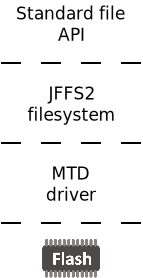
\includegraphics[width=\textwidth]{slides/sysdev-flash-filesystems/jffs2.pdf}
  \end{columns}
\end{frame}

\begin{frame}
  \frametitle{jffs2 - How to use}
  On the Linux {\bf target}
  \begin{itemize}
  \item Need either the \code{mtd-utils} package from the MTD project,
    or their embedded variants from Busybox
  \item Erase and format a partition with jffs2:\\
    \code{flash_eraseall -j /dev/mtd2}
  \item Mount the partition:\\
    \code{mount -t jffs2 /dev/mtdblock2 /mnt/flash}\\
  \item Fill the contents by writing\\
    (copying from NFS or from external storage)
  \item Other possibility: use a {\em jffs2} image (see next page to
    produce it):\\
    \code{flash_eraseall /dev/mtd2}\\
    \code{nandwrite -p /dev/mtd2 rootfs.jffs2}
  \end{itemize}
\end{frame}

\begin{frame}
  \frametitle{How to create a jffs2 image}
  \begin{itemize}
  \item \code{mkfs.jffs2} command available in the mtd-utils package.\\
    Caution: unlike some \code{mkfs} commands, it doesn't create a
    filesystem, but a filesystem image.
  \item First, find the erase block size (on the target running Linux):\\
    \code{cat /proc/mtd} \\
    For example: \code{00040000} (256 KiB)
  \item Then create the image on your workstation:\\
    \code{mkfs.jffs2 --pad --no-cleanmarkers --eraseblock=256 -d rootfs/ -o rootfs.jffs2}
  \item The \code{--pad} option pads the jffs2 image contents\\
    until the end of the final erase block.
  \item It is fine if the jffs2 image is smaller than the MTD partition.\\
    The jffs2 file system will use the entire partition anyway.
  \item The \code{--no-cleanmarkers} option is for NAND flash only.
  \end{itemize}
\end{frame}

\begin{frame}
  \frametitle{Mounting a jffs2 image on your host}
  Useful to edit \code{jffs2} images on your development system\\
  Mounting an MTD device as a loop device is a bit complex task.\\
  Here's an example for \code{jffs2}, for your reference:
  \begin{itemize}
  \item First find the erase block size used to create the jffs2 image.\\
    Let's assume it is 256KiB (262144 bytes).
  \item Create a block device from the image\\
    \code{losetup /dev/loop0 root.jffs2}
  \item Emulate an MTD device from a block device,\\
    using the \code{block2mtd} kernel module\\
    \code{modprobe block2mtd block2mtd=/dev/loop0,262144}
  \item Load the mtdblock driver if needed\\
    \code{modprobe mtdblock}
  \item Finally, mount the filesystem (create \code{/mnt/jffs2} if needed)\\
    \code{mount -t jffs2 /dev/mtdblock0 /mnt/jffs2}
  \end{itemize}
\end{frame}

\begin{frame}
  \frametitle{Initializing jffs2 partitions from U-boot}
  You may not want to have \code{mtd-utils} on your target!
  \begin{itemize}
  \item Create a JFFS2 image on your workstation
  \item In the U-Boot prompt:
    \begin{itemize}
    \item Download the jffs2 image to RAM with \code{tftp}\\
      Or copy this image to RAM from external storage\\
      (U-boot understands FAT filesystems and supports USB storage)
    \item Flash it inside an MTD partition\\
      (exact instructions depending on flash type, NOR or NAND,\\
      reuse the instructions used to flash your kernel). Make sure to
      write only the size of the image, not more!
    \item If you boot on a jffs2 root filesystem, add
      \code{root=/dev/mtdblock<x>} and \code{rootfstype=jffs2} to the
      Linux command line arguments.
    \end{itemize}
  \item Limitation: need to split the jffs2 image in several chunks\\
    if bigger than the RAM size.
  \end{itemize}
\end{frame}

\begin{frame}
  \frametitle{yaffs2}
  \begin{columns}
    \column{0.7\textwidth}
    \begin{itemize}
    \item Mainly supports NAND flash
    \item No compression
    \item Wear leveling, ECC, power failure resistant
    \item Fast boot time
    \item Code available separately through git\\
      (Dual GPL / Proprietary license\\
      for non Linux operating systems)
    \item \url{http://www.yaffs.net/}
    \end{itemize}
    \column{0.3\textwidth}
    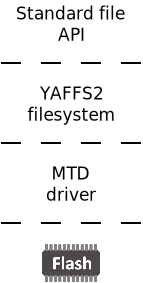
\includegraphics[width=\textwidth]{slides/sysdev-flash-filesystems/yaffs2.pdf}
  \end{columns}
\end{frame}

\begin{frame}
  \frametitle{yaffs2 - How to use}
  \begin{itemize}
  \item Erase a partition:\\
    \code{flash_eraseall /dev/mtd2}
  \item The filesystem is automatically formatted at the first mount:\\
    \code{mount -t yaffs2 /dev/mtdblock2 /mnt/flash}
  \item Images can be created with the \code{mkyaffs} tool, from \code{yaffs-utils}\\
    \url{http://code.google.com/p/yaffs2utils/}
  \end{itemize}
\end{frame}

\begin{frame}
  \frametitle{UBI (1)}
  Unsorted Block Images
  \begin{itemize}
  \item \url{http://www.linux-mtd.infradead.org/doc/ubi.html}
  \item Volume management system on top of MTD devices.
  \item Allows to create multiple logical volumes and spread writes
    across all physical blocks.
  \item Takes care of managing the erase blocks and wear
    leveling. Makes filesystems easier to implement.
  \item Wear leveling can operate on the whole storage,
    not only on individual partitions (strong advantage). 
  \item Volumes can be dynamically resized or, on the opposite, can be
    read-only (static).
  \end{itemize}
\end{frame}

\begin{frame}
  \frametitle{UBI (2)}
  \begin{center}
    \includegraphics[width=\textwidth]{slides/sysdev-flash-filesystems/ubi.pdf}
  \end{center}
\end{frame}

\begin{frame}
  \frametitle{UBIFS}
  \begin{columns}
    \column{0.7\textwidth}
    \url{http://www.linux-mtd.infradead.org/doc/ubifs.html}
    \begin{itemize}
    \item The next generation of the jffs2 filesystem, from the same
      linux-mtd developers.
    \item Available since Linux 2.6.27
    \item Works on top of UBI volumes
    \item Has a noticeable metadata overhead on very small partitions
      (4M, 8M)
    \end{itemize}
    \column{0.3\textwidth}
    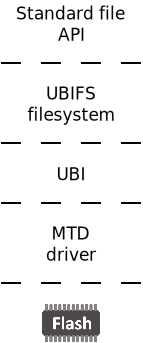
\includegraphics[width=\textwidth]{slides/sysdev-flash-filesystems/ubifs.pdf}
  \end{columns}
\end{frame}

\begin{frame}
  \frametitle{UBI layout example}
  \begin{center}
    \includegraphics[width=\textwidth]{slides/sysdev-flash-filesystems/ubifs-layout.pdf}
  \end{center}
\end{frame}

\begin{frame}
  \frametitle{UBI - Preparation}
  \begin{itemize}
  \item Have \code{/dev/} mounted as a \code{devtmpfs} filesystem
  \item Erase your flash partition while preserving your erase counters\\
    \code{ubiformat /dev/mtd1}\\
    See \url{http://www.linux-mtd.infradead.org/faq/ubi.html} if you
    face problems
  \item Attach UBI to one (of several) of the MTD partitions:\\
    \code{ubiattach /dev/ubi_ctrl -m 1}
  \item This command creates the \code{ubi0} device, which represent
    the full UBI space stored on MTD device 1 (new \code{/dev/ubi0}
    character device)
  \end{itemize}
\end{frame}

\begin{frame}
  \frametitle{UBI - Volume management}
  \begin{itemize}
  \item Volume creation with \code{ubimkvol}
    \begin{itemize}
    \item \code{ubimkvol /dev/ubi0 -N test -s 116MiB}
    \item \code{ubimkvol /dev/ubi0 -N test -m} (max available size)
    \item The volume is then identified as \code{ubi0:test} for the
      \code{mount}/\code{umount} commands
    \end{itemize}
  \item Volume removal with \code{ubirmvol}
    \begin{itemize}
    \item \code{ubirmvol /dev/ubi0 -N test}
    \end{itemize}
  \end{itemize}
\end{frame}

\begin{frame}
  \frametitle{UBIFS - How to use}
  \begin{itemize}
  \item When a UBI volume is created, creating an empty UBIFS
    filesystem is just a matter of mounting it
    \begin{itemize}
    \item \code{mount -t ubifs ubi0:test /mnt/flash}
    \end{itemize}
  \item Images of UBIFS filesystems can be created using the
    \code{mkfs.ubifs} utility
    \begin{itemize}
    \item \code{mkfs.ubifs -m 4096 -e 256KiB -c 1000 -r rootfs/ ubifs.img}
      \begin{itemize}
      \item \code{-m 4096}, minimal I/O size\\
                 (see \code{/sys/class/mtd/mtdx/writesize}).
      \item \code{-e 252 KiB}, logical erase block size (smaller than
                 PEB size, look at \code{dmesg})
      \item \code{-c 1000}, maximum number of logical erase
        blocks. Details:
        {\tiny\url{http://linux-mtd.infradead.org/faq/ubifs.html\#L_max_leb_cnt}}
      \end{itemize}
    \item Can be written to a UBI volume using \code{ubiupdatevol} and
      the \code{/dev/ubiX_Y devices}
    \end{itemize}
  \end{itemize}
\end{frame}

\begin{frame}
  \frametitle{Ubinize}
  \begin{itemize}
  \item Images of a full UBI space, containing several volumes can be
    created using the \code{ubinize} utility
    \begin{itemize}
    \item Can be written to a raw MTD partition using \code{nand write} in U-boot.
    \item Caution: \code{nand erase} will also erase the Erase
      Counters
    \end{itemize}
  \item \code{ubinize -o ubi.img -p 256KiB -m 4096 ubi.ini}
    \begin{itemize}
    \item Creates \code{ubi.img}, with 256KiB physical erase blocks,
      4096 minimum I/O size (\code{-m}).
    \end{itemize}
  \item Build systems like Buildroot can do this for you!
  \end{itemize}
\end{frame}

\begin{frame}[fragile]
  \frametitle{UBIFS - How to prepare a root fs}
  \begin{itemize}
  \item Create the UBIFS image from the target directory
  \item Write the configuration file for the UBI device (\code{ubi.ini}):
\small
\begin{verbatim}
[RFS-volume]
mode=ubi
image=rootfs.ubifs
vol_id=1
vol_size=30MiB
vol_type=dynamic
vol_name=rootfs
vol_flags=autoresize
vol_alignment=1
\end{verbatim}
\normalsize
  \item Create the UBI device image
  \item Flash it using a bad block aware command from the bootloader
  \item Pass UBI layout information to the kernel:
    \begin{itemize}
    \item \code{rootfstype=ubifs ubi.mtd=1 root=ubi0:rootfs}
    \end{itemize}
  \end{itemize}
\end{frame}

\begin{frame}
  \frametitle{Flash filesystem benchmarks}
  \url{http://elinux.org/Flash_Filesystem_Benchmarks}
  \begin{itemize}
  \item {\bf jffs2}
    \begin{itemize}
    \item Worst performance
    \item Requires \code{CONFIG_SUMMARY} to have acceptable boot time
    \end{itemize}
  \item {\bf yaffs2}
    \begin{itemize}
    \item Good performance, but not in mainline Linux
    \end{itemize}
  \item {\bf ubifs}
    \begin{itemize}
    \item Best solution and performance for medium and big
      partitions
    \item Too much metadata overhead small partitions (only case
      when \code{yaffs2} and \code{jffs2} are still useful)
    \end{itemize}
  \end{itemize}
\end{frame}

\begin{frame}
  \frametitle{Issues with flash-based block storage}
  \begin{itemize}
  \item Flash storage made available only through a block interface.
  \item Hence, no way to access a low level flash interface
    and use the Linux filesystems doing wear leveling.
  \item No details about the layer (Flash Translation Layer) they
    use. Details are kept as trade secrets, and may hide poor
    implementations.
  \item Hence, it is highly recommended to limit the number of writes
    to these devices.
  \end{itemize}
\end{frame}

\begin{frame}
  \frametitle{Reducing the number of writes}
  \begin{itemize}
  \item Of course, do not use your flash storage as swap area (rare in
    embedded systems anyway)
  \item Mount your filesystems as read-only, or use read-only
    filesystems (SquashFS), whenever possible.
  \item Keep volatile files in RAM (tmpfs)
  \item Don't use the \code{sync} mount option (commits writes
    immediately). Use the \code{fsync()} system call for per-file
    synchronization.
  \item You may decide to do without journaled filesystems. They cause
    more writes, but are also much more power down resistant
    (trade-off).
  \end{itemize}
\end{frame}

\begin{frame}
  \frametitle{Useful reading}
  \begin{itemize}
  \item Arnd Bergmann: Optimizing Linux with cheap flash drives\\
    In depth coverage of flash storage with a block interface.\\
    \url{http://lwn.net/Articles/428584/}
  \item Introduction to JFFS2 and LogFS:\\
    \url{http://lwn.net/Articles/234441/}
  \item Nice UBI presentation from Toshiba:\\
    \url{http://free-electrons.com/redirect/celf-ubi.html}
  \item Documentation on the linux-mtd website:\\
    \url{http://www.linux-mtd.infradead.org/}
  \end{itemize}
\end{frame}

\setuplabframe
{Flash Filesystems}
{
  \begin{itemize}
  \item Creating partitions in your internal flash storage.
  \item Use a read-only JFFS2 partition for the system
  \item Use a read-write JFFS2 partition for data
  \end{itemize}
}
